\documentclass[12pt,thmsa]{article}
\usepackage[french,english]{babel}
\usepackage[ansinew]{inputenc}
\usepackage[T1,OT1]{fontenc}
\usepackage{graphicx}
\usepackage{amsmath,amssymb,listings}
\usepackage{alltt,algorithmic,algorithm}
\usepackage{multicol}
\usepackage{cite}
\usepackage{fancyhdr}
\usepackage{setspace}
\usepackage{array}
\usepackage{amsfonts}
\usepackage{latexsym}
\usepackage{epsf}
\usepackage{umlaute}
\usepackage{setspace}
\usepackage{amsthm}
\usepackage{enumerate}


\setlength{\textwidth}{160mm}
\setlength{\textheight}{230mm}
\setlength{\oddsidemargin}{-5mm}
\setlength{\topmargin}{-10mm}

% to get rid of the numbers in the bibliography:
\makeatletter
\def\@biblabel#1{}
\makeatother



\title{Assignement 3}



\begin{document}


\noindent \textsc{University of Geneva}     \hfill \textsc{Bachelor in Economics and Management} \\
\textbf{Probability 1}                      \hfill \textsc{Bachelor in International Relations} \\
Professor Davide La Vecchia                 \hfill Spring 2018  \\
ASSIGNMENT 03                               \hfill   March 13th



\noindent
\makebox[\linewidth]{\rule{\textwidth}{0.4pt}}\\[1.5ex]

\section*{Exercise 1}


The mail order company `CD-Bill' sends a questionnaire to households
in its address file to know if they are interested in rap,
classical or rock  music, genres in which it is specialized. By searching the answers, it
notes that 20\% of households are not interested in any of these 3 genres of music, 35\% of households are interested in rap, 20\% in classical music and the number of households interested in rock is twice as many as in classical music. In addition, 5\%
households are interested in both rap and rock and no household is interested in
both rap and classical music.

%\medskip

\begin{itemize}
\item $Rap$: rap music;
\item $Class$: classcal music;
\item $Rock$: rock music.

The information given in the statement can be rewritten in a formal way:

\begin{itemize}
\item $P(\overline{Rap}\cap\overline{Class}\cap\overline{Rock})=0.20$;
\item $P(Rap)=0.35$;
\item $P(Class)=0.20$;
\item $P(Rock)=2P(Class)= 0.40$;
\item $P(Rap\cap Rock)=0.05$;
\item $P(Rap\cap Class)=0$.
%\item $P(Rap\cap Class\cap Rock)=0$
\end{itemize}
%\medskip

We immediately deduce that $P(Rap\cap Class\cap Rock)=0$.\\


\medskip
\noindent Before proceeding, it is often very useful to graph all of these information in a classic Venn diagram:\footnote{Note that here, the area of intersection between $Rap$ and $Class$ should be non-existent to be perfectly correct, since $P(Rap\,\cap\, Class)=0$.}\\
\begin{center}
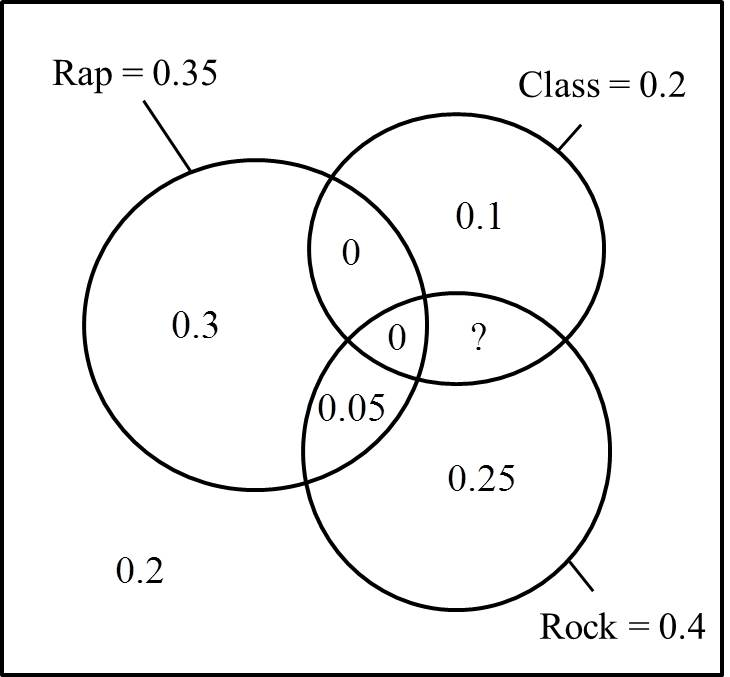
\includegraphics[scale=0.8]{Graph1.jpg}
\end{center}


\end{itemize}
\noindent If one randomly chooses one of the households that responded to the
  survey:

 \begin{enumerate}%[(a)]
 \item What is the probability that he/she is interested in rap or
classical music?

We use the fact that $P(A \cup B)=P(A)+P(B)-P(A \cap B)$:
\begin{center} $P(Rap \cup Class)=P(Rap)+P(Class)-P(Rap \cap Class)= 0.35+0.20-0=0.55.$ \end{center}


 \item What is the probability that he/she is interested in rock, knowing
that they are interested in rap?

We use the conditional probability $P(A \mid B)=\dfrac{P(A \,\cap\, B)}{P(B)}$:
\begin{center} $P(Rock \mid Rap)=\dfrac{P(Rock \,\cap\, Rap)}{P(Rap)}=\dfrac{0.05}{0.35}=0.1429.$ \end{center}

 \item What is the probability that he/she is interested in at least 2 kinds of
music ?

Let's name the event that he/she is interested in at least 2 kinds of music by $AM 2$.
Event $AM 2$, in the Venn diagram, corresponds to the surface of the three-leaf clover formed by the intersection of the three musical styles (i.e. the union of the intersections of the genres). So, formally,
\begin{center} $AM2 = (Rap \cap Class)\cup(Class \cap Rock)\cup(Rock \cap Rap).$ \end{center}
We can therefore use the probability of union of two events: \begin{center} $P(A \cup B)=P(A)+P(B)-P(A \cap B)$ \end{center} and generalize it for three events
\footnote{Or proceed by steps:
\begin{center} $P((Rap \cap Class)\cup(Class \cap Rock)\cup(Rock \cap Rap))=P((Rap \cap Class)\cup(Class \cap Rock))+P(Rock \cap Rap)- P(((Rap \cap Class)\cup(Class \cap Rock))\cap (Rock \cap Rap)$.
\end{center}

Or, $(Rap \cap Class)\cup(Class \cap Rock)$=$(Class \cap Rock)$ because $(Rap \cap Class)=\emptyset$.


So $(Rap \cap Class)\,\cup\,(Class \cap Rock))\,\cap\, (Rock \cap Rap) = (Class \cap Rock)\,\cap\, (Rock \cap Rap)=(Class \cap Rock \cap Rap)=\emptyset$.


Finally,
\begin{center} $P((Rap \cap Class)\cup(Class \cap Rock))\cup(Rock \cap Rap))= P((Rap \cap Class)\cup(Class \cap Rock))+P(Rock \cap Rap)$\\
Or $(Rap \cap Class)\cup(Class \cap Rock)=(Class \cap Rock)$ car $(Rap \cap Class)=\emptyset$.
\end{center}

So 
\begin{center}$P((Rap \cap Class)\cup(Class \cap Rock))\cup(Rock \cap Rap))= P(Class \cap Rock)+P(Rock \cap Rap)$.
\end{center}
}:
$$
P(A \cup B \cup C) = P(A) + P(B) + P(C) - P(A \cap B) - P(A \cap C) - P(B
\cap C) + P(A \cap B \cap C).
$$
% \medskip

Here, $A=(Rap \cap Class)$; $B=(Class \cap Rock)$ and $C=(Rock \cap Rap)$.


We have a special case: $(A \cap B) = (A \cap C) = (B \cap C)=(A \cap B \cap C)$.

In this situation, we will have: $P(A \cup B \cup C) = P(A) + P(B) + P(C) - 2P(A \cap B \cap C)$.



\begin{center}
$P((Rap \cap Class)\cup(Class \cap Rock)\cup(Rock \cap Rap)) = P(Rap \cap Class) + P(Class \cap Rock) + P(Rock \cap Rap)$ - $2P((Rap \cap Class) \cap (Class \cap Rock) \cap (Rock \cap Rap))= P(Class \cap Rock) + P(Rock \cap Rap)$.
\end{center}



Because $P((Rap \cap Class))=0$ and $P((Rap \cap Class) \cap (Class \cap Rock) \cap (Rock \cap Rap))=P(Rap\cap Class\cap Rock)=0$.
%\medskip

We do not know $P(Class \cap Rock)$, so it must  be calculated. 
%\medskip

We know that:
\begin{eqnarray*}
P(Rap \cup Rock \cup Class) &=& P(Rap) + P(Rock) + P(Class) - P(Rap \cap
Rock)\\&& - P(Rock \cap Class) - P(Rap \cap Class) + P(Rap \cap Rock \cap
Class)\\
&=& 0.35+0.40+0.20-0.05-P(Rock \cap Class)-0+0\\
& =& 0.9 - P(Rock \cap Class)
\end{eqnarray*}
and
$$
       P(Rap \cup Rock \cup Class) = 1 -
       P(\overline{Rap}\cap\overline{Class}\cap\overline{Rock}) = 1-0.2=0.8.
$$
% \smallskip

So $P(Rock \cap Class)=0.1$, and we can calculate:
\begin{center} $P(AM2)=0.1+0.05=0.15.$ \end{center}

 \item What is the probability that he/she is interested in rap, knowing that he/she is interested in neither classical nor rock music?
 \end{enumerate}

We have
$$
P(Rap \mid \overline{Class}\,\cap\, \overline{Rock})=1-P(\overline{Rap} \mid \overline{Class}\,\cap \,\overline{Rock})=1-
\frac{P(\overline{Rap} \,\cap\, \overline{Class} \,\cap\,
\overline{Rock})}{P(\overline{Class}\,\cap\, \overline{Rock})}
$$
with
$P(\overline{Class}\cap \overline{Rock})=1-P(Class \cup
Rock)=1-P(Class)-P(Rock)+P(Class \cap Rock)=1-0.2-0.4+0.1=0.5.$\\


So $ P(Rap \mid \overline{Class}\cap \overline{Rock})$=$1-\dfrac{0.2}{0.5}=0.6$.

\section*{Exercise 2}


Roger Federer prepares for Wimbledon tennis tournament to get
a new victory. Since turf is the best surface, we know that regardless of the player he faces, the probability of winning a match is 0.85. To win the tournament a player has to win seven consecutive games.

We define the Event $G_i$: `Win i matches'
\begin{enumerate} %[(a)]

\item What is the probability that Federer reaches at least the semi-finals?

In order to reach the semifinals, Federer must have won the quarter-finals, i.e. he must have won 5 consecutive games\footnote{The $7_{th}$ match is the final, the $6_{th}$ semifinal, the $5_{th}$ quarterfinals.}.
\begin{center} $P(G_5)=0.85^5=0.4437$.
\end{center}

\item Federer reached the quarter-finals (5th round). What is the probability that he wins the tournament?

We use the conditional probability:
\begin{center} $P(G_7 \mid G_4)= \dfrac{P(G_7 \,\cap\, G_4)}{P(G_4)}=\dfrac{P(G_7)}{P(G_4)}=\dfrac{0.85^7}{0.85^4}=0.85^3$ = $0.6141.$
\end{center}

Note: $P(G_7 \cap G_4)$=$P(G_7)$ since Event $G_7$ is included in $G_4$: $G_7 \subset G_4$. It simply means that it is not possible to win the final without first reaching the quarter-finals.

\item A sports commentator says that if Novak Djokovic is in the final with Federer, the latter has a 60\% chance of winning the tournament against 90\% if Djokovic does not qualify.
 He says Djokovic has a 75\% chance of reaching the final. Calculate the probability that Federer wins the tournament according to this person (assuming he is in the final).

Let's define the events:
\begin{itemize}
\item $DF$: Djokovic reaches the final;
\item $FED$: Federer wins the tournament.
\end{itemize}

We know \begin{itemize} \item $P(FED \mid DF)=0.6$; \item $P(FED \mid \overline{DF})=0.9$; \item $P(DF)=0.75$. \end{itemize}

The total probability of Event $FED$ is
$$
P(FED)=P(FED \mid DF)\cdot P(DF) + P(FED \mid \overline{DF}) \cdot
P(\overline{DF})
$$
So
$$P(FED)= 0.6\cdot 0.75 + 0.9\cdot 0.25 = 0.45+0.225 = 0.675.$$ 
\end{enumerate}

\section*{Exercise 3}

The probability that a new car battery works for over  30'000km is
0.8, the probability that it functions for over 60'000km is 0.4, and the probability that it
works for over 90'000km is 0.1. If a new car battery is still working after 30'000km,
what is the probability that

\begin{enumerate}
\item  its total life will exceed 60'000km?
\item its additional life will exceed 60'000km?

\end{enumerate} 

\noindent Solutions:\\
We define Variable B: `battery life of a new car in km'. We have the information that:
\begin{itemize}
\item $P(B> 30000) =0.8$;
\item $P(B>60000) = 0.4$;
\item $P(B>90000)=0.1$.
\end{itemize}

\begin{enumerate}
\item We have \begin{align*}
P(B > 60000 \mid B > 30000) = \frac{ P(B > 60000 \cap B> 30000) }{ P(B > 30000) }= \frac{P(B>60000) }{P(B > 30000)}= \frac{0.4}{0.8}= 0.5.
\end{align*}

\item 
\noindent We know $B - 30000 > 60000 \Leftrightarrow B>90000$. So
\begin{align*}
P( B > 90000 \mid B>30000 ) =  \frac{ P(B > 90000 \cap B> 30000) }{ P(B > 30000) }= \frac{P(B>90000) }{P(B > 30000)}= \frac{0.1}{0.8}= 0.125.
\end{align*}
\end{enumerate}

 
\section*{Exercise 4}
Consider the random experiment of tossing a fair coin twice. Let us define the following events:
\begin{itemize}
\item $ A $: Observe a head $ (H) $ on the first toss
\item $ B $: Observe a head $ (H) $ on the second toss
\item $ C $: Observe the same outcome on both tosses
\end{itemize}
Are the events pairwise independent? Are the events jointly independent?\\
\noindent Solutions:\\
The sample set is $ S=\{HH, HT, TH, TT\} $ with each outcome being equally likely. Now, rewrite $ A_{1}=\{HH, HT\} $, $ A_{2}=\{HH, TH\} $, $ A_{3}=\{HH, TT\} $. Thus we have $ P(A_{1})=P(A_{2})=P(A_{3})=1/2 $. Now we have $ P(A_{1} \cap A_{2})=P(HH)=1/4=P(A_{1})P(A_{2}) $, That is the two events $ A_{1}, A_{2} $ are independent. Similarly, one should can verify that $ A_{1}, A_{3} $ and $ A_{2}, A_{3} $ are independent. To the contrary, $ P(A_{1}\cap A_{2} \cap A_{3})=P(HH)=1/4 $, is not the same as $ P(A_{1})P(A_{2})P(A_{3}) $.



\section*{Exercise 5 (Optional)}


Given the axioms of probability theory, show the following:
\begin{enumerate}
  \item $P(\emptyset)=0$
  \item $P(A^c)=1-P(A)$
  \item $P(A \cap B) \leq \min(P(A),P(B))$
  \item $P(A \cup B)=P(A)+P(B)-P(A \cap B)$
  \item If $A_1, A_2,...$ are mutually exclusive events in $\mathcal{B}$, then
\begin{equation}
P\left(  \bigcup_{i=1}^{n} A_i \right) = \sum_{i=1}^{n} P(A_i).  \label{Eq: ProbUnionDisj}
\end{equation}
  \item Let's $A_n$ a collection of sets such that: $\lim_{n\rightarrow \infty}A_n= A$.
  Show that $\lim_{n\rightarrow \infty}P(A_n)=P(A)$.
\end{enumerate}

Tip: we can use Venn diagram to prove the above.










\end{document}



